
\documentclass{article}

\usepackage[margin=1.33in]{geometry}
\usepackage{p200}
\usepackage[colorlinks=true,linkcolor=blue]{hyperref}

\hypersetup{pdftitle = {Physics 203 Course Syllabus} }
\hypersetup{pdfauthor = {}, pdfsubject = {Physics} }

\pagestyle{plain}

\begin{document}

\begin{center}
{\LARGE Physics 203 Syllabus}
\vskip 0.25cm
{\large The microscopic source of force}

\vskip 0.25cm
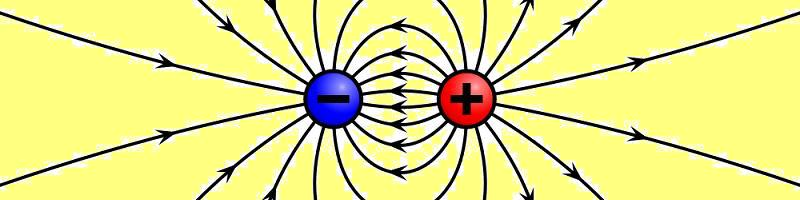
\includegraphics[width=\textwidth]{c:/Users/Dave/Desktop/repos/github/spot/content/banners/203.jpg}

\vskip 0.25cm
{\large Summer 2013}
\end{center}

\begin{center}
\renewcommand{\arraystretch}{1.5}
\renewcommand{\tabcolsep}{0.2cm}
\begin{tabular}{ll}
\hline
Instructor & David J. Ulrich \\




Campus & PCC Rock Creek, Bldg 7 \\ 
Room & 223/225 \\ 
Time & 6:00 pm \\ 
\hline
\end{tabular}
\end{center}

\section{Course Overview}

%
This course will cover such topics as electromagnetism, relativity, quantum mechanics and nuclear science.
%
In addition, we will touch on some subjects related to solid state physics and particle physics.
%
%

%
Our textbook will be \emph{Physics (9th edition)} by Cutnell and Johnson.
%
We will be covering chapters 18--24 and 28--32 in this course.
%
%

Each Monday session will be held in Room 223. This room contains the material used for the labs. Therefore labs will fall on the Monday meetings. The Wednesday sessions will consist solely in lecture and will be held in Room 225.

This class rocks!



\section{Intended Outcomes}

After completion of this course, students will

%
\begin{itemize}

\item Apply knowledge of electricity, magnetism, and modern physics to explain natural physical processes and related technological advances.

\item Use an understanding of algebraic mathematics along with physical principles to effectively solve problems encountered in everyday life, further study in science, and in the professional world.

\item Design experiments and acquire data in order to explore physical principles, effectively communicate results, and critically evaluate related scientific studies.

\item Assess the contributions of physics to our evolving understanding of global change and sustainability while placing the development of physics in its historical and cultural context.

\end{itemize}





\section{Grading Scheme}

Your total grade will be a weighted average of all the assignments in class. The weight for each category of assignments is in the following table.

\begin{center}

\renewcommand{\arraystretch}{1.5}
\renewcommand{\tabcolsep}{0.2cm}

\begin{tabular}{lc}
\hline
\textbf{Category} & \textbf{Weight} \\
\hline

Exam & 50\% \\

Quiz & 25\% \\

Lab & 25\% \\

\hline
\end{tabular}

\end{center}



\clearpage





\section{Class Schedule}

This following schedule should be considered tentative. Based on class progress, we may slow down or speed up the schedule.

\begin{center}

\renewcommand{\arraystretch}{1.5}
\renewcommand{\tabcolsep}{0.2cm}

\begin{tabular}{@{}cccp{16mm}p{64mm}@{}}
%\begin{tabular}{cccll}
\hline
\textbf{Wk} &
\textbf{Day} &
\textbf{Date} &
\textbf{Type} &
\textbf{Title} &
\hline

1 &
Mon &
Jun 24 &
Lecture 1 &
Electric Field and Potential \\

1 &
Wed &
Jun 26 &
Lab 1 &
Projectiles and Free-Fall \\

\hline
\end{tabular}

\end{center}

\clearpage





\section{Course Content}

%
\begin{itemize}

\item ELECTRIC FORCES AND FIELDS
%
\begin{itemize}

\item Study the forces between charges and apply Coulomb's Law to solve problems.

\item Distinguish insulators and conductors.

\item Understand charging by conduction and induction and explain the action of an electroscope to illustrate these.

\item Plot electric fields about various charge configurations, thereby coming to understand the basic concept of an electric field.

\end{itemize}

\item ELECTRIC POTENTIAL
%
\begin{itemize}

\item Explain electrical potential energy and to show how it is analogous to gravitational potential energy.

\item Explain the central importance of potential difference as ``electrical pressure'' that moves charge.

\item Relate work and potential difference, and thereby understand and define the volt.

\item Explain the role of batteries as energy sources and as sources of potential difference.

\item Define the electron volt as an energy unit.

\item Explain the operation of capacitors, including charging and discharging, dielectrics and the energy stored therein.

\end{itemize}

\item DIRECT CURRENT CIRCUITS
%
\begin{itemize}

\item Discuss the concept of electric current and what is happening at the atomic level.

\item Explain Ohm's Law and how it operates in both simple and complex circuits.

\item Explain resistivity and resistance and relate the two.

\item Explain the effect of resistors in series, parallel and series-parallel circuits and solve related problems.

\item Discuss the effect of capacitors in series, parallel and series-parallel circuits and solve related problems.

\item State and apply Kirchhoff's Junction Rule.

\item State and apply Kirchhoff's Loop Rule.

\item Describe the construction and operation of galvanometers, ammeters and voltmeters.

\item Describe ``house'' circuits and discuss electrical safety.

\end{itemize}

\item MAGNETISM
%
\begin{itemize}

\item Plot magnetic fields and understand their nature by analogy to electric fields.

\item Explain the magnetic fields caused by electric currents.

\item Discuss the force on a current in a magnetic field and be able to calculate its magnitude and determine its direction from the Right Hand Rule.

\item Explain the Hall effect.

\item Diagram and explain the earth's magnetic field.

\item Describe lines of flux and understand flux density.

\item Define Ampere's Law.

\item Compute the magnitude and direction of the magnetic fields about a current loop, a solenoid and a taroid.

\item Explain the torque on a current loop in a magnetic field and how this is used in electric meters.

\end{itemize}

\item ELECTROMAGNETIC INDUCTION
%
\begin{itemize}

\item Define induced EMFs.

\item Explain mutual induction and self induction.

\item Explain the characteristics of an inductance-resistance circuit.

\item Explain motional EMFs.

\item Describe the theory and operation of an AC generator and how it can be converted to a DC generator.

\item Describe the theory and operation of an electric motor.

\item Describe the theory and operation of a transformer.

\end{itemize}

\item ALTERNATING CURRENTS AND ELECTRONICS
%
\begin{itemize}

\item Define AC quantities such as peak, effective and RMS values.

\item Apply Ohm's Law to an AC resistive circuit.

\item Explain the charging and discharging of capacitors and show how capacitors fit into an AC circuit.

\item Explain the inductance and inductive reactance of a coil and how coils fit into AC circuits.

\item Apply Ohm's law to problem solving in a combined RCL circuit.

\item Explain the phenomenon of electrical resonance.

\item Explain the phenomenon of thermionic emission.

\item Explain the diode, the semiconductor diode and rectification.

\item Discuss various electronic devices such as the x-ray machine, oscilloscope, etc.

\end{itemize}

\item ELECTROMAGNETIC WAVES
%
\begin{itemize}

\item Explain the generation of EM waves.

\item Discuss the reception of radio waves.

\item Discuss the speed of EM waves.

\item Diagram and explain the EM spectrum.

\item Describe the ability of EM waves to transport energy.

\end{itemize}

\item MODERN PHYSICS
%
\begin{itemize}

\item Identify the circumstances, discoveries and people that launched Modern Physics.

\item Enumerate and understand the postulate of relativity.

\item Learn about the speed of light as a natural limit to speed.

\item Explain the problem of simultaneity and calculate time changes from one frame of reference to another.

\item Describe relativistic length contraction.

\item Describe the relativistic mass-energy relation.

\item Explain the work of Planck and Compton.

\item Explain the uncertainty principle and the other features of Quantum Mechanics.

\end{itemize}

\item ATOMIC STRUCTURE AND THE EMISSION OF EM ENERGY
%
\begin{itemize}

\item Identify the nuclear atom and the Bohr model.

\item Describe the spectrum of hydrogen and to show how the Bohr model can be used to explain its emission.

\item Draw energy level diagrams.

\item Explain absorption of light by the Bohr model.

\item Relate De Broglie's waves to the Bohr atom.

\item Describe Quantum numbers and the Pauli exclusion principle.

\item Explain the production of x-rays and the principle of the x-ray machine.

\item Summarize our knowledge of bright line, band, absorption and continuous spectra.

\end{itemize}

\item THE NUCLEUS
%
\begin{itemize}

\item Describe the structure of atomic nuclei.

\item Explain the formation of isotopes

\item Relate mass defect and binding energy.

\item Explain the phenomena of radioactivity including decay products and radioactive series.

\item Explain nuclear reactions and transmutations.

\item Explain the nuclear force.

\item Describe nuclear fission and explain how this relates to bombs and reactors.

\item Describe nuclear fusion and explain how this relates to bombs and reactors.

\item Explain radiation damage and radiation detection.

\item Summarize the known nuclear particles including the probable quarks.

\end{itemize}

\end{itemize}

\clearpage



\end{document}